\documentclass[tikz,border=6pt]{standalone}
\usepackage{amsmath}
\usetikzlibrary{arrows.meta,calc,patterns,positioning}
\begin{document}

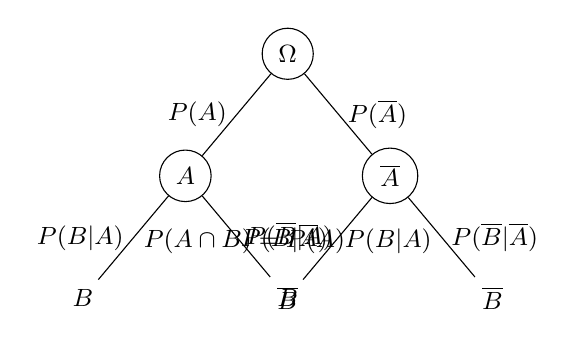
\begin{tikzpicture}[>=Latex,level distance=1.55cm,sibling distance=2.6cm,
  every node/.style={font=\small}]
  \node[circle,draw] {$\Omega$}
    child {node[circle,draw] {$A$}
      child {node {$B$} edge from parent node[left] {$P(B|A)$}}
      child {node {$\overline B$} edge from parent node[right] {$P(\overline B|A)$}}
      edge from parent node[left] {$P(A)$}}
    child {node[circle,draw] {$\overline A$}
      child {node {$B$} edge from parent node[left] {$P(B|\overline A)$}}
      child {node {$\overline B$} edge from parent node[right] {$P(\overline B|\overline A)$}}
      edge from parent node[right] {$P(\overline A)$}};
  \node[below=2.1cm] at (0,0) {$P(A\cap B)=P(A)P(B|A)$};
\end{tikzpicture}

\end{document}
